Un jugador del kino elige sus 15 numeros antes del juego. en el sorteo se salen seleccionados 15 numeros de 25 que hay en la t\'ombola,
donde se gana premio si se acierta a 11, 12, 13, 14 o 15 de los n\'umeros.
% son 15 numeros
% se eligen 15 de 25
% premio si acierta 11,12,14 o 15
%
% Es hipergeometrica  X ~ Hipergeo(n,m,l) 
% n = 25 Numeros Totales
% m = 15 Numeros que eligen de los 25
% l = 15 Numeros que tomamos
\begin{itemize} 
	\item ?`Cu\'al es la cantidad esperada y varianza de aciertos que tenga el jugador en el sorteo?\\
		$Esperanza\ =\ E(x)\ =\ \frac{l\cdot m}{n}\ =\ \frac{15\cdot 15}{25}\ =\ 9$\\
		$Varianza\ =\ V(x)\ =\ \frac{l\cdot m\cdot (n-m)\cdot (n-l)}{n^{2}\cdot (n-1)}\ =\ \frac{15\cdot 15\cdot (25-15)\cdot (25-15)}{25^{2}\cdot (25-1)}\ =\ 1.5$\\
	\item ?`Cu\'al es la probabilidad de que el jugador logre 11 aciertos?\\
		% $P(X=11)\ =\ \frac{{m\choose 11}{10\choose 4}}{{25\choose 15}}\ =\ 0.1436782\ =\ 14.4\%$\\ % dhyper(11,15,15,25)
		$P(X=11) = \frac{{15 \choose 11}{10 \choose 4}}{{25\choose 15}} = 0.0876938$
		% dhyper(11,15,10,15)
		% dhyper(x,m,n,k) Teniendo m cosas tipo 1, n cosas tipo 2, probabilidad de sacar x del tipo n, al tomar k del conjunto
	\item ?`Cu\'al es la probabilidad de que no gane premio el jugador?\\
		$P(X<=10)\ = \sum_{i=0}^{10} \frac{{15 \choose i}{10 \choose 15-i}}{{25\choose 15}}   =\ 0.894111$\\
		% phyper(10,15,10,15)
	\item ?`Cu\'al es la probabilidad de que acierte a los 15 numeros?\\
		$P(X=15)\ = \frac{{15 \choose 15}{10 \choose 0}}{{25\choose 15}} = 3.059264*10^{-7}$\\
		%dhyper(15,15,10,15)
	\item Realice gr\'aficos de la funci\'on de densidad de probabilidad y de la funci\'on de distribuci\'on.\\
		% x<-seq(1,25)   % sera 1,15 ? :S
	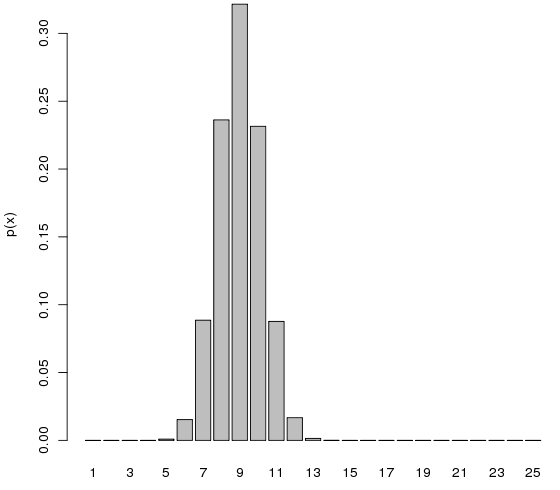
\includegraphics[scale=0.5]{images/1_5-dhyper}\\		% barplot(dhyper(x,15,10,15),names.arg=x)
	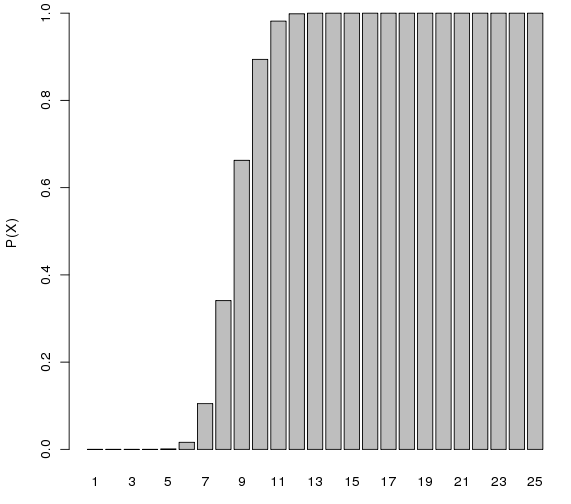
\includegraphics[scale=0.5]{images/1_5-phyper}		% barplot(phyper(x,15,10,15),names.arg=x)
	\item Var\'ie el o los valores de los par\'ametros de la distribuci\'on y comente lo observado en los gr\'aficos de la funci\'on de densidad y de distribuci\'on. (2 casos).\\
	
	\begin{itemize}
		\item Funci\'on de Densidad\\
			Variando la cantidad de bolitas totales (35 bolitas):\\
		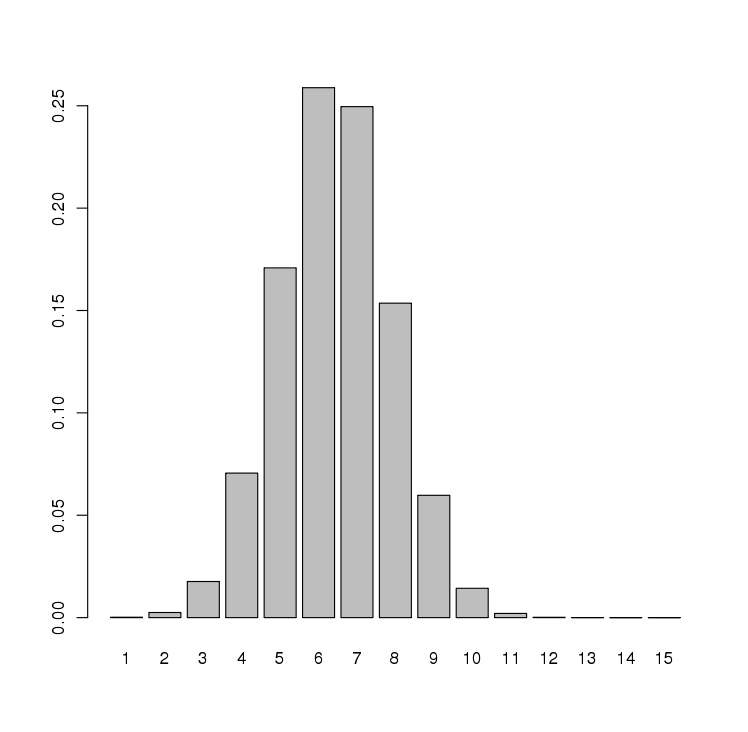
\includegraphics[scale=0.5]{images/1_5-dhyper-variado1}\\
			Variando la cantidad de bolitas totales (55 bolitas):\\
		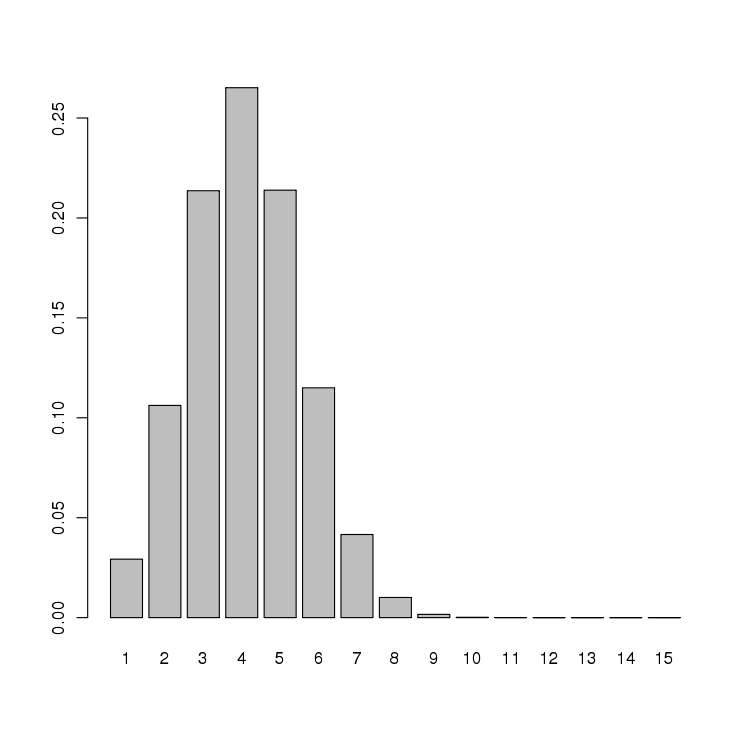
\includegraphics[scale=0.5]{images/1_5-dhyper-variado2}\\
		Finalmente, podemos concluir que a mayor cantidad de bolitas, la probabilidad de obtener algun premio disminuye considerablemente.\\
		\item Funci\'on de Distribuci\'on\\
			Variando la cantidad de bolitas totales (35 bolitas):\\
		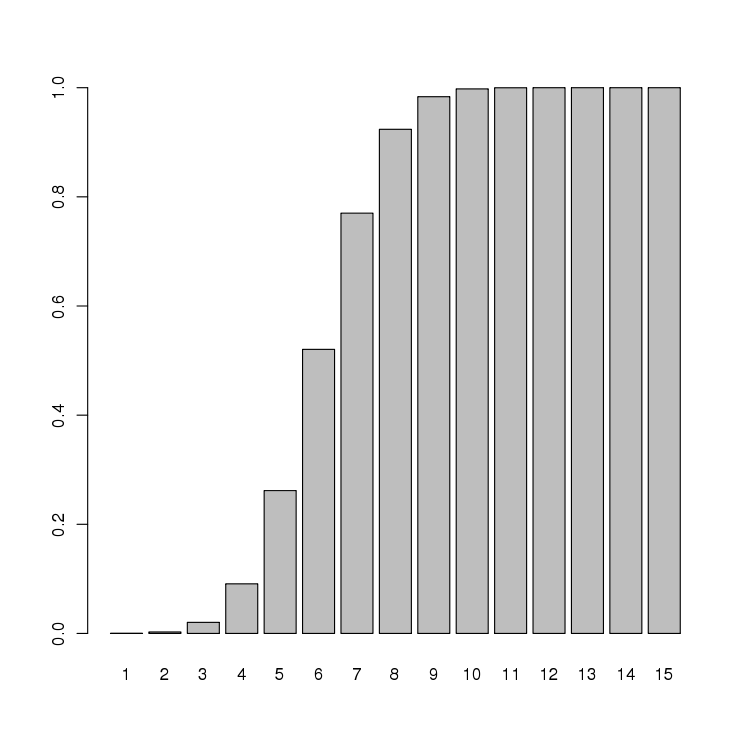
\includegraphics[scale=0.5]{images/1_5-phyper-variado1}\\
			Variando la cantidad de bolitas totales (55 bolitas):\\
		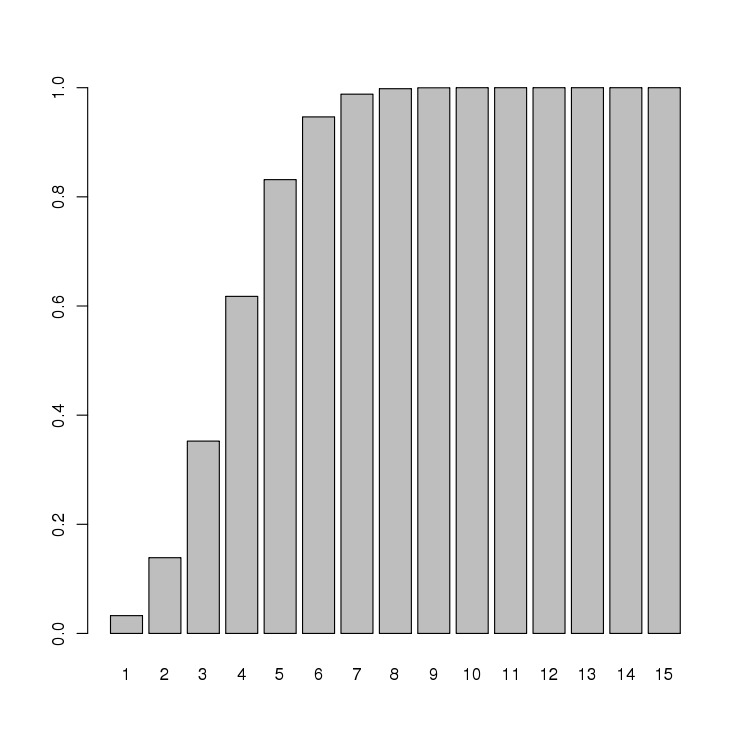
\includegraphics[scale=0.5]{images/1_5-phyper-variado2}\\
		En conclusion, con respecto a aumentar la cantidad de bolitas, podemos observar que aumenta la probabilidad de obtener menores resultados.\\
	\end{itemize}

\end{itemize}
